\documentclass[xcolor=dvipsnames]{beamer}

\usepackage[utf8]{inputenc}
\usepackage{amsmath,amssymb}
\usepackage{textpos}

%\usepackage[usenames,dvipsnames]{xcolor}
\usepackage{tikz}
\usetikzlibrary{patterns}
\usetikzlibrary{calc}
\usetikzlibrary{decorations.pathmorphing}
\usepackage{pgfplots}

\definecolor{LTMBlue}{RGB}{0,51,102}

% \usepackage{ifthen}
% \newboolean{showsectionpage} % Boolean showsectionpage definieren
% \setboolean{showsectionpage}{false} % Section-Seiten anzeigen (true) oder nicht (false)
% \usetheme{fau-4-3}

\usefonttheme{professionalfonts} % Schriftsatz ändern
\pdfpageattr {/Group << /S /Transparency /I true /CS /DeviceRGB>>} 
\setbeamertemplate{navigation symbols}{}

\setbeamercolor{frametitle}{fg=LTMBlue,bg=White}
\addtobeamertemplate{frametitle}{}{%
\begin{textblock*}{100mm}(.95\textwidth,-0.75cm)

\includegraphics[height=0.5cm]{LTM_Logo_klein}
\end{textblock*}}

\title[LKM Demos]{LKM Demos}
\author[Jan Friederich, Paul Steinmann]{Jan Friederich, Paul Steinmann}
\date{\today}
\institute[LTM]{Chair of Applied Mechanics}
% \logo{
\includegraphics[height=5mm]{LTM_Logo_klein}}

\renewcommand{\v}[1]{\boldsymbol{#1}}

\pgfplotsset{compat=newest}
\pgfplotsset{verticalbar/.style={
    xmin=0.0,xmax=0.1,ymin=0.0,ymax=0.1,
%     xshift=3.5cm,yshift=1.3cm,scale=0.4,
    hide axis,
    scale only axis,
    height=0,
    width=0,
    title style={at(1,1), anchor=south west, font=\normalsize},
    colormap={}{rgb255(0cm)=(0,0,255) rgb255(0.75cm)=(0,255,255)
      rgb255(1.5cm)=(0,255,0) rgb255(2.25cm)=(255,255,0) rgb255(3cm)=(255,0,0)},
    colorbar,% sampled,
    colorbar style={
 	font=\footnotesize,
% 	samples=16,
	scaled y ticks=false,
	/pgf/number format/fixed,
	extra y ticks={\pgfkeysvalueof{/pgfplots/ymin},\pgfkeysvalueof{/pgfplots/ymax}},
	extra y tick style={yticklabel style={xshift=-0.7em, anchor=east}},
        height=3cm,
        width=0.3cm,
        xshift=-1.0cm,
        yshift=0cm
    },
  }
}
% \pgfplotsset{horizontalbar/.style={
%     hide axis,
%     scale only axis,
%     height=0pt,
%     width=0pt,
%     colormap={}{rgb255(0cm)=(0,0,255) rgb255(1cm)=(0,255,255)
%       rgb255(3cm)=(255,255,0) rgb255(4cm)=(255,0,0)},
%     colorbar horizontal,
%     colorbar style={
% % 	font=\scriptsize,
%         height=0.4cm,
%         width=4cm,
% %         xshift=-2cm,
% %         yshift=-1.9cm
%     }
%   }
% }

\begin{document}

\begin{frame}
 \frametitle{Demo 1-1 $\vert$ \bfseries Elastostatics}
 \framesubtitle{\bfseries prescribed surface tractions}
 \begin{overlayarea}{0.9\textwidth}{0.9\textheight}
%  \vspace*{1ex}
 \begin{center}
 \begin{tikzpicture}[scale=2]
  \onslide<1>{
  \fill[gray!10, draw=black] (0, 1) rectangle (3, 0) node[above left, black]{$\mathcal{B}$};
  }

  \onslide<1>{
  \draw[thin,gray] (0, 0) -- +(0, -0.5);
  \draw[thin,gray] (3, 0) -- +(0, -0.5);
  \draw[<->,thin,gray] (0, -0.4) -- node[fill=white]{$3 \ell$} +(3, 0);
  \draw[thin,gray] (3, 0) -- +(0.5, 0);
  \draw[thin,gray] (3, 1) -- +(0.5, -0);
  \draw[<->,gray] (3.4, 0) -- node[fill=white,sloped]{$\ell$} +(0, 1);

   \draw[thick,-latex] (0,0) -- +(0.5, 0) node[below]{$\v e_1$};
   \draw[thick,-latex] (0,0) -- +(0, 0.5) node[right]{$\v e_2$};
  }
  
  \onslide<1>{
  \foreach \x in {0.0, 0.25,0.5,...,2.75, 3.0}
  \draw[-latex] (0.05+2.9/3.0*\x, 1.5) -- +(0, -0.5);  
%   \draw (0.05, 1.5) -- node[above]{$10 \,\mathrm{MPa}$} +(2.9, 0);
  \draw (0.05, 1.5) -- +(2.9, 0);
  \node at (2.9, 1.5) [right,xshift=0.1cm]{$\v t^p$};
  }

  \onslide<2>{
  \node at(1.5,0.4) {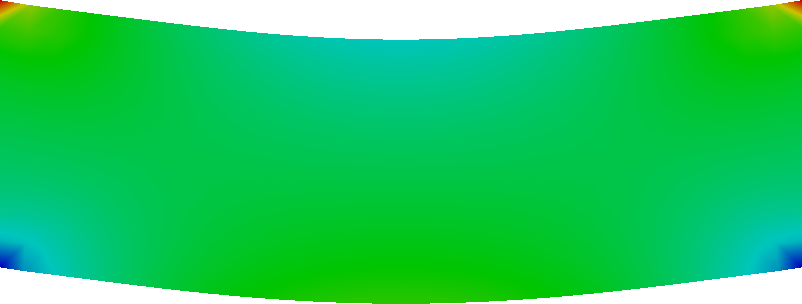
\includegraphics[width=6cm]{../01-elasto-static/01-tractions/plot_11.png}};
  \begin{scope}[xshift=3.5cm,yshift=1.3cm,scale=0.5]
   \begin{axis}[verticalbar,point meta min=-7.2,point meta max=10.3,title={$\sigma_{11}$ in $\mathrm{MPa}$}] 
    \addplot [draw=none] coordinates {(0,0)}; \end{axis}
  \end{scope}   
  }
  \onslide<3>{
  \node at(1.5,0.4) {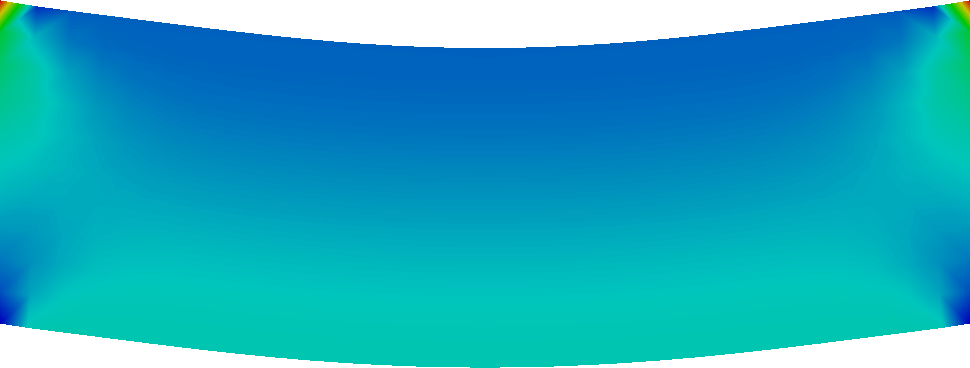
\includegraphics[width=6cm]{../01-elasto-static/01-tractions/plot_22.png}};
  \begin{scope}[xshift=3.5cm,yshift=1.3cm,scale=0.5]
   \begin{axis}[verticalbar,point meta min=-1.87,point meta max=5.09,title={$\sigma_{22}$ in $\mathrm{MPa}$}] 
    \addplot [draw=none] coordinates {(0,0)}; \end{axis}
  \end{scope}   
  }
  \onslide<4>{
  \node at(1.5,0.4) {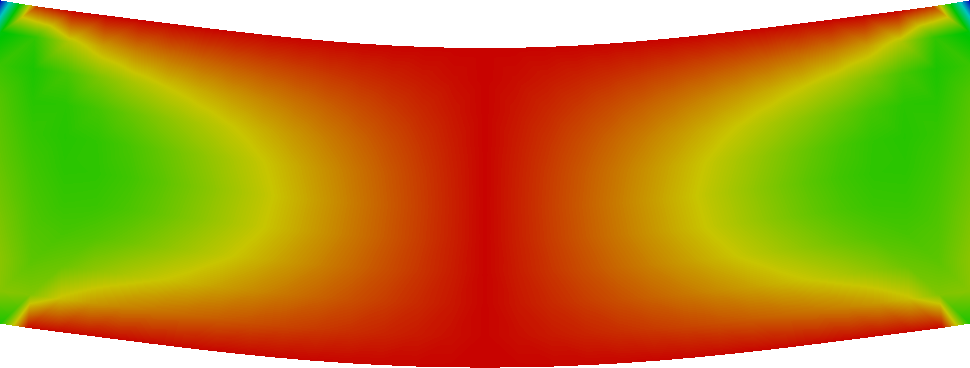
\includegraphics[width=6cm]{../01-elasto-static/01-tractions/plot_12.png}};
  \begin{scope}[xshift=3.5cm,yshift=1.3cm,scale=0.5]
   \begin{axis}[verticalbar,point meta min=-3.75,point meta max=0.02,title={$\sigma_{12}$ in $\mathrm{MPa}$}] 
    \addplot [draw=none] coordinates {(0,0)}; \end{axis}
  \end{scope}   
  }

  \onslide<1-4>{
  \fill[pattern=north west lines, pattern color=black] (0, -0.25) rectangle +(-0.25, 1.5);
  \draw[thick] (0, -0.25) -- +(0, 1.5);
  \fill[pattern=north west lines, pattern color=black] (3, -0.25) rectangle +(0.25, 1.5);
  \draw[thick] (3, -0.25) -- +(0, 1.5);
  }
  
  \begin{scope}
   \onslide<1>{\node at (0, -1) [right]{\parbox{3cm}{$E = 200 \, \mathrm{GPa}$ \\ $\nu = 0.3$ \\ $\ell = 1\,\mathrm{m}$}};}
   \onslide<1>{\node at (1.5, -1) [right]{$[t^p_i] = -\begin{bmatrix} 0 \\ 1 \\ 0 \end{bmatrix} \mathrm{MPa}$ on $\partial \mathcal{B}^t_\text{top}$};}
   \onslide<2-4>{\node at (0, -0.5) [right,font=\footnotesize]{$\v u$ scaled with a factor of $5000$};}
  \end{scope}
  
  \end{tikzpicture}
  \end{center}

 \end{overlayarea}
\end{frame}

% 
% \begin{frame}
%  \begin{tikzpicture}
%    \node at(0,0) {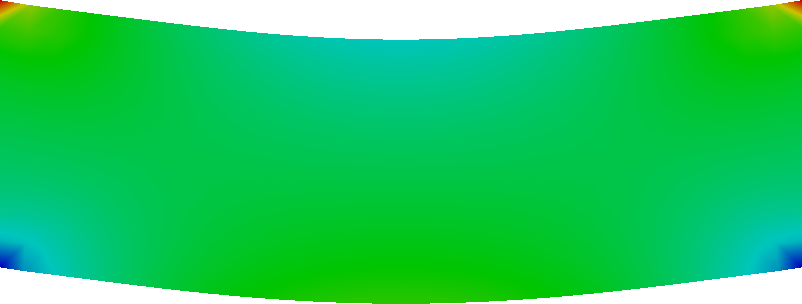
\includegraphics[width=6cm]{../01-elasto-static/01-tractions/plot_11.png}};
%    \begin{axis}[verticalbar,point meta min=-7.2,point meta max=10.3] \addplot [draw=none] coordinates {(0,0)}; \end{axis}
%    \draw (0, 0) node[above right, xshift=0cm,yshift=0cm]{$\sigma_{11}$ in $\mathrm{MPa}$};
%  \end{tikzpicture}
% \end{frame}
% 

\begin{frame}
 \frametitle{Demo 1-2 $\vert$ \bfseries Elastostatics}
 \framesubtitle{\bfseries volume forces}
 \begin{overlayarea}{0.9\textwidth}{0.9\textheight}
%  \vspace*{1ex}
 \begin{center}
 \begin{tikzpicture}[scale=2]
  \onslide<1>{
  \fill[gray!10, draw=black] (0, 1) rectangle (3, 0) node[above left, black]{$\mathcal{B}$};
  }

  \onslide<1>{
  \draw[thin,gray] (0, 0) -- +(0, -0.5);
  \draw[thin,gray] (3, 0) -- +(0, -0.5);
  \draw[<->,thin,gray] (0, -0.4) -- node[fill=white]{$3 \ell$} +(3, 0);
  \draw[thin,gray] (3, 0) -- +(0.5, 0);
  \draw[thin,gray] (3, 1) -- +(0.5, -0);
  \draw[<->,gray] (3.4, 0) -- node[fill=white,sloped]{$\ell$} +(0, 1);

   \draw[thick,-latex] (0,0) -- +(0.5, 0) node[below]{$\v e_1$};
   \draw[thick,-latex] (0,0) -- +(0, 0.5) node[right]{$\v e_2$};
  }
  
  \onslide<1>{
%   \foreach \x in {0.0, 0.25,0.5,...,2.75, 3.0}
%   \draw[-latex] (0.05+2.9/3.0*\x, 1.5) -- +(0, -0.5);  
%   \draw (0.05, 1.5) -- node[above]{$10 \,\mathrm{MPa}$} +(2.9, 0);
%   \node at (2.9, 1.5) [right,xshift=0.1cm]{$\v t^p$};
   \draw[-latex,thick] (1.5, 0.5) -- node[right] {$\v b$} +(0, -0.4);
  }

  \onslide<2>{
  \node at(1.5,0.4) {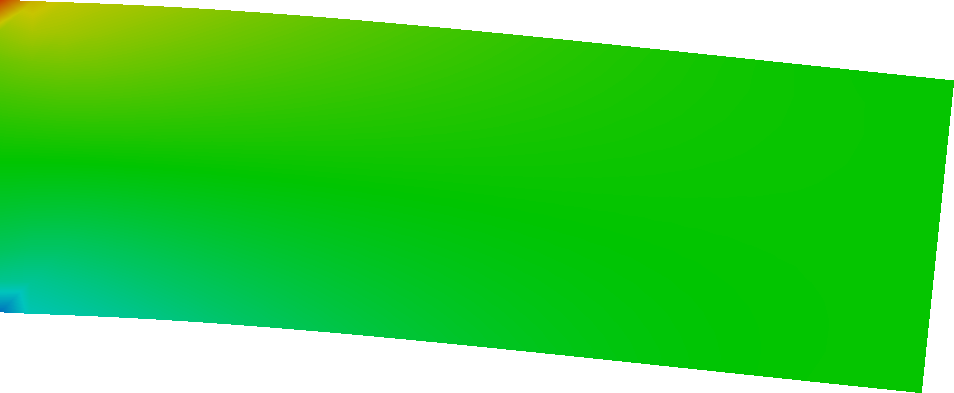
\includegraphics[width=6cm]{../01-elasto-static/02-gravity/plot_11.png}};
  \begin{scope}[xshift=3.5cm,yshift=1.2cm,scale=0.5]
   \begin{axis}[verticalbar,point meta min=-4.04,point meta max=3.94,title={$\sigma_{11}$ in $\mathrm{MPa}$}]
   \addplot [draw=none] coordinates {(0,0)}; \end{axis}
  \end{scope}   
  }
  \onslide<3>{
  \node at(1.5,0.4) {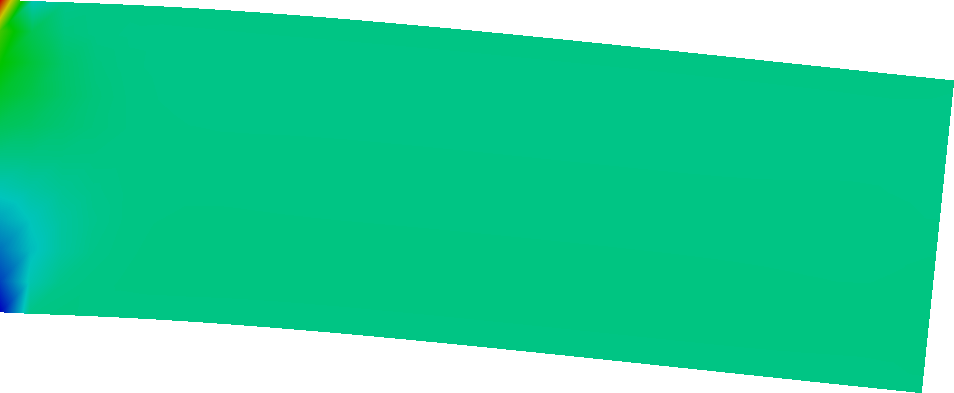
\includegraphics[width=6cm]{../01-elasto-static/02-gravity/plot_22.png}};
  \begin{scope}[xshift=3.5cm,yshift=1.2cm,scale=0.5]
   \begin{axis}[verticalbar,point meta min=-0.774,point meta max=1.6,title={$\sigma_{22}$ in $\mathrm{MPa}$}]
   \addplot [draw=none] coordinates {(0,0)}; \end{axis}
  \end{scope}   
  }
  \onslide<4>{
  \node at(1.5,0.4) {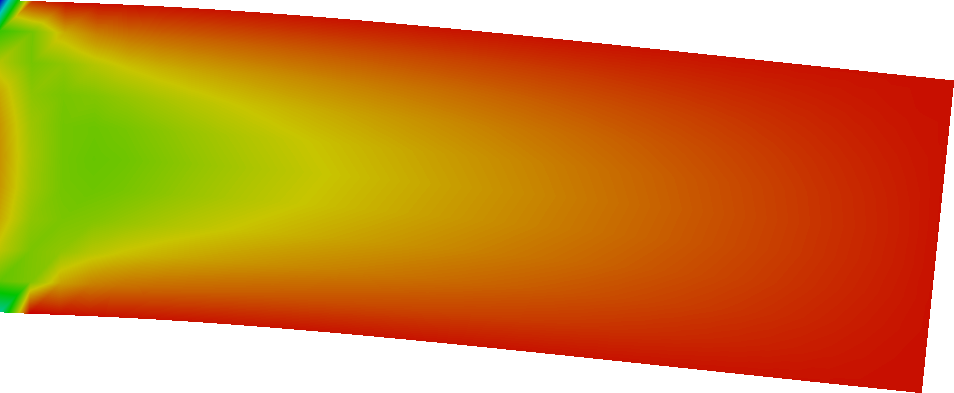
\includegraphics[width=6cm]{../01-elasto-static/02-gravity/plot_12.png}};
  \begin{scope}[xshift=3.5cm,yshift=1.2cm,scale=0.5]
   \begin{axis}[verticalbar,point meta min=-0.0209,point meta max=0.02,title={$\sigma_{12}$ in $\mathrm{MPa}$}]
   \addplot [draw=none] coordinates {(0,0)}; \end{axis}
  \end{scope}   
  }
  
  \onslide<1-4>{
  \fill[pattern=north west lines, pattern color=black] (0, -0.25) rectangle +(-0.25, 1.5);
  \draw[thick] (0, -0.25) -- +(0, 1.5);
%   \fill[pattern=north west lines, pattern color=black] (3, -0.25) rectangle +(0.25, 1.5);
%   \draw[thick] (3, -0.25) -- +(0, 1.5);
  }

  \begin{scope}
   \onslide<1>{\node at (0, -1) [right]{\parbox{3cm}{$E = 200 \, \mathrm{GPa}$ \\ $\nu = 0.3$ \\ $\ell = 1\,\mathrm{m}$}};}
   \onslide<1>{\node at (1.5, -1) [right]{\parbox{3cm}{$\v b = - \rho \, g \, \v e_2$ \\ $\rho = 8000 \, \mathrm{kg}/\mathrm{m}^3$ \\ $g = 9.81 \, \mathrm{N}/\mathrm{kg}$}};}
   \onslide<2-4>{\node at (0, -0.5) [right,font=\footnotesize]{$\v u$ scaled with a factor of $5000$};}
  \end{scope}
  
  \end{tikzpicture}
  \end{center}

 \end{overlayarea}
\end{frame}


\begin{frame}
 \frametitle{Demo 1-3 $\vert$ \bfseries Elastostatics}
 \framesubtitle{\bfseries prescribed displacements}
 \begin{overlayarea}{0.9\textwidth}{0.9\textheight}
%  \vspace*{1ex}
 \begin{center}
 \begin{tikzpicture}[scale=2]
%  \draw[draw=none] (-1, -2) rectangle (8, 2);
  \onslide<1>{
  \fill[gray!10, draw=black] (0, 1) rectangle (3, 0) node[above left, black]{$\mathcal{B}$};
  }

  \onslide<1>{
  \draw[thin,gray] (0, 0) -- +(0, -0.5);
  \draw[thin,gray] (3, 0) -- +(0, -0.5);
  \draw[<->,thin,gray] (0, -0.4) -- node[fill=white]{$3 \ell$} +(3, 0);
  \draw[thin,gray] (3, 0) -- +(0.7, 0);
  \draw[thin,gray] (3, 1) -- +(0.7, -0);
  \draw[<->,gray] (3.6, 0) -- node[fill=white,sloped]{$\ell$} +(0, 1);

   \draw[thick,-latex] (0,0) -- +(0.5, 0) node[below]{$\v e_1$};
   \draw[thick,-latex] (0,0) -- +(0, 0.5) node[right]{$\v e_2$};
  }
  
  \onslide<1>{
%   \foreach \x in {0.0, 0.25,0.5,...,2.75, 3.0}
%   \draw[-latex] (0.05+2.9/3.0*\x, 1.5) -- +(0, -0.5);  
%   \draw (0.05, 1.5) -- node[above]{$10 \,\mathrm{MPa}$} +(2.9, 0);
%   \node at (2.9, 1.5) [right,xshift=0.1cm]{$\v t^p$};
%    \draw[-latex,thick] (1.5, 0.5) -- node[right] {$\v b = - \rho \, g \, \v e_3$} +(0, -0.4);
    \draw[thick,dashed] (3,0.5) -- +(0.5,0.0);
    \draw[thick,-latex] (3.3,0.3) arc[x radius=0.1, y radius=0.4, start angle=-10, end angle=190] node[below right,xshift=1mm]{$\v u^p$};
  }

 \onslide<2>{
  \node at(1.5,0.4) {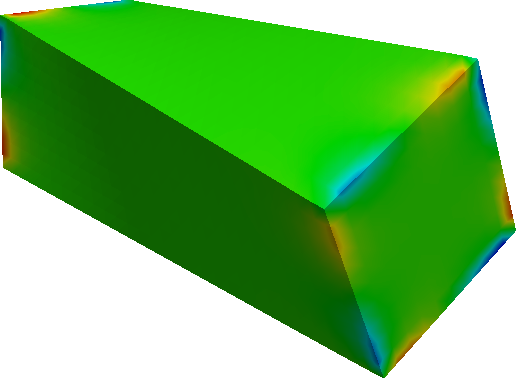
\includegraphics[width=6cm]{../01-elasto-static/03-rotation/plot_11.png}};
  \begin{scope}[xshift=3.5cm,yshift=1.2cm,scale=0.5]
   \begin{axis}[verticalbar,point meta min=-511,point meta max=440,title={$\sigma_{11}$ in $\mathrm{MPa}$}]
   \addplot [draw=none] coordinates {(0,0)}; \end{axis}
  \end{scope}   
  }
  \onslide<3>{
  \node at(1.5,0.4) {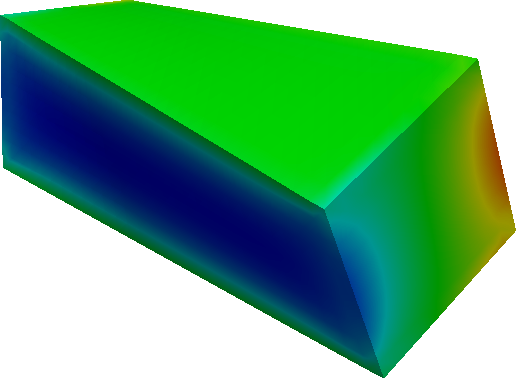
\includegraphics[width=6cm]{../01-elasto-static/03-rotation/plot_12.png}};
  \begin{scope}[xshift=3.5cm,yshift=1.2cm,scale=0.5]
   \begin{axis}[verticalbar,point meta min=-306,point meta max=306,title={$\sigma_{12}$ in $\mathrm{MPa}$}]
   \addplot [draw=none] coordinates {(0,0)}; \end{axis}
  \end{scope}   
  }
  \onslide<4>{
  \node at(1.5,0.4) {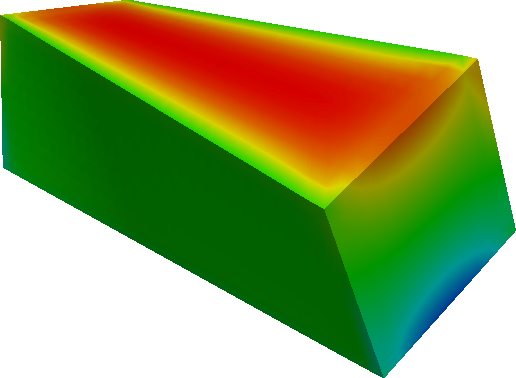
\includegraphics[width=6cm]{../01-elasto-static/03-rotation/plot_13.png}};
  \begin{scope}[xshift=3.5cm,yshift=1.2cm,scale=0.5]
   \begin{axis}[verticalbar,point meta min=-306,point meta max=306,title={$\sigma_{13}$ in $\mathrm{MPa}$}]
   \addplot [draw=none] coordinates {(0,0)}; \end{axis}
  \end{scope}   
  }
  
  \onslide<2-4>{
   \draw[gray,thick,-latex] (0.02,0.52) -- +(0.4, -0.22) node[below] {$\v e_1$};
   \draw[gray,thick,-latex] (0.02,0.52) -- +(-0.02, 0.45) node[left] {$\v e_2$};
   \draw[gray,thick,-latex] (0.02,0.52) -- +(-0.4, -0.15) node[below] {$\v e_3$};
  }
  
  \onslide<1>{
  \fill[pattern=north west lines, pattern color=black] (0, -0.25) rectangle +(-0.25, 1.5);
  \draw[thick] (0, -0.25) -- +(0, 1.5);
%   \fill[pattern=north west lines, pattern color=black] (3, -0.25) rectangle +(0.25, 1.5);
%   \draw[thick] (3, -0.25) -- +(0, 1.5);
  }

  \begin{scope}%[yshift=-1cm]
   \onslide<1>{\node at (0, -1) [right]{\parbox{3cm}{$E = 200 \, \mathrm{GPa}$ \\ $\nu = 0.3$ \\ $\ell = 1\,\mathrm{m}$}};}
   \onslide<1>{\node at (1.5, -1) [right]{$\v u^p :$ ``rotate by $1^\circ$'' on $\partial \mathcal{B}^u_\text{right}$};}
   \onslide<2-4>{\node at (0, -1) [right,font=\footnotesize]{$\v u$ scaled with a factor of $30$};}
  \end{scope}
  
  \end{tikzpicture}
  \end{center}

 \end{overlayarea}
\end{frame}

% \begin{frame}
%  \frametitle{Demo 1-1 $\vert$ \bfseries Elastostatics}
%   \begin{center}
%   \begin{tikzpicture}[scale=2]
%   \node at(1.5,0.35) {\includegraphics[width=6cm]{../01-elasticity-static/01.png}};
% %   \node at(0,0) {$\v \sigma_{11}$};
% 
%   \fill[pattern=north west lines, pattern color=black] (0, -0.25) rectangle +(-0.25, 1.5);
%   \draw[thick] (0, -0.25) -- +(0, 1.5);
%   \fill[pattern=north west lines, pattern color=black] (3, -0.25) rectangle +(0.25, 1.5);
%   \draw[thick] (3, -0.25) -- +(0, 1.5);
%   
%   \begin{scope}[xshift=1.5cm,yshift=-1.3cm,scale=0.35]
%    \begin{axis}[horizontalbar,point meta min=-100,point meta max=100] \addplot [draw=none] coordinates {(0,0)}; \end{axis}
%    \draw (0, 0) node[above right, xshift=0cm,yshift=0.2cm]{$\sigma_{11}$ in $\mathrm{MPa}$};
%   \end{scope}   
% 
%   \end{tikzpicture}
%  \end{center}
% \end{frame}

\end{document}
